\documentclass{article}
\usepackage[utf8]{inputenc}
\usepackage{enumitem}
\usepackage{graphicx}

\begin{document}

\section*{Steps for Data Processing Workflow}

\begin{figure}[h!]
    \centering
    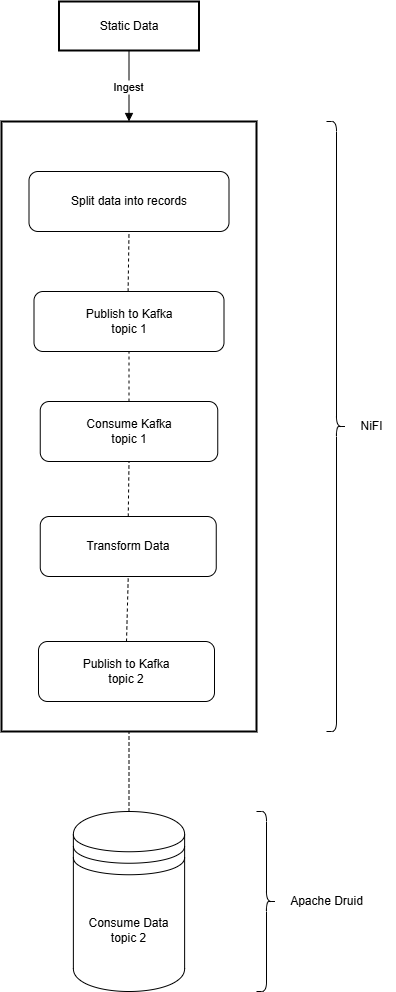
\includegraphics[width=0.5\textwidth]{ETL.png}
    \caption{ETL Workflow Diagram}
    \label{fig:etl_diagram}
\end{figure}


\begin{enumerate}
    \item \textbf{Initial Ingestion of Static Data:}
    \begin{itemize}
        \item NiFi ingests \texttt{tracking\_data\_x.xlsx} and \texttt{tracking\_data\_y.json} as static files.
        \item NiFi can read these files from the directory \texttt{data\_input/incoming}.
        \item The xlsx file will be converted to json in Nifi
    \end{itemize}

    \item \textbf{Record-by-Record Processing with NiFi:}
    \begin{itemize}
        \item After loading the entire dataset, NiFi splits each file into individual rows (or records in the case of JSON data).
        \item Each row/record will be processed individually, treating each one as a separate message to simulate real-time data.
        \item The FirstInFirstOut Prioritizer is used to move data in the order that it comes in.
    \end{itemize}

    \item \textbf{Add Delay Between Records:}
    \begin{itemize}
        \item The \texttt{ControlRate} processor in NiFi is used to introduce a 1-second delay between records.
        \item This delay simulates a real-time data stream by pacing the flow of messages instead of sending them all at once.
    \end{itemize}

    \item \textbf{Send Records to Kafka:}
    \begin{itemize}
        \item NiFi’s \texttt{PublishKafka} processor sends each delayed message to a Kafka topic (\texttt{tracking\_data}).
        \item This creates a continuous stream of data in Kafka, where each record arrives approximately every second.
    \end{itemize}

    \item \textbf{Data Transformation:}
    \begin{itemize}
        \item NiFi's \texttt{ConsumeKafka} consumes messages from the \texttt{tracking\_data} topic.
        \item The dataset's schemas for both datasets are combined, and the newly formed dataset is transformed.
        \item The transformed data is published to Kafka in a new topic(\texttt{publish\_tracking\_druid}).
    \end{itemize}

    \item \textbf{Load Data to Time-Series DB:}
    \begin{itemize}
        \item Apache Druid consumes messages from the Kafka topic(\texttt{publish\_tracking\_druid}) in real-time data streaming.
    \end{itemize}
\end{enumerate}

\end{document}
